\begin{frame}
	\frametitle{Sign flip}
	\begin{tikzpicture}[
	expl/.style={draw=black, thick=2pt,fill=blue!20,rounded corners},
	arrow/.style={red!80!black,ultra thick,->,>=latex}]	
	\node[anchor=south west,inner sep=0] (image) at (0,0) {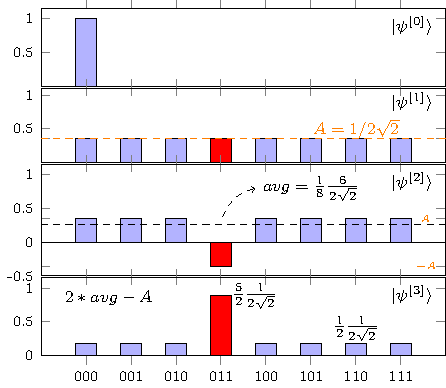
\includegraphics[width=0.5\textwidth]{figures/bar-graph/probs.pdf}};
	\begin{scope}[x={(image.south east)},y={(image.north west)}]
	%\draw[help lines,xstep=.1,ystep=.1] (0,0) grid (1,1);
	%\foreach \x in {0,1,...,9} { \node [anchor=north] at (\x/10,0) {0.\x}; }
	%\foreach \y in {0,1,...,9} { \node [anchor=east] at (0,\y/10) {0.\y}; }
	\node[expl](A) at (1.5,0.875) {\Large Initial state $\ket{\psi^{[0]}}$};
	\node[expl](B) at (1.5,0.65) {\Large Initialization $\ket{\psi^{[1]}}$};
	\node[expl](C) at (1.5,0.4) {\Large Sign flip $\ket{\psi^{[2]}}$};
	\node[expl](D) at (1.5,0.15) {\Large Inversion about average $\ket{\psi^{[3]}}$};
	
	\draw[arrow] (A.south) -- node [right]{Hadamard $H$} (B.north);
	\draw[arrow] (B.south) -- node [right]{Oracle $U_f$} (C.north);
	\draw[arrow] (C.south) -- node [right]{Difussion $U_d$} (D.north);
	\draw[thick,dashed] (0.01,0.3) rectangle (1.85,0.75);
	\draw[arrow] (D.north east) to[bend right] node [right]{$\frac{\pi}{4}\sqrt{n}$} (B.east);
	\end{scope}	
	\end{tikzpicture}	
\end{frame}
\begin{frame}
	\frametitle{Sign flip}
	We find a method (unitary operator) which flip the sign of the state of interest.
	\pause
	\begin{block}{\textit{Quantum Oracle}}
		It is defined the operator $U_f$: 
		\[U_{f}:\left.|j\right\rangle _{n}\otimes\left.|y\right\rangle _{1}\rightarrow\left.|j\right\rangle _{n}\otimes\left.|y\oplus f\left(j\right)\right\rangle _{1},\]
		where $\oplus$ is the sum operator in mod 2, and $f\left(j\right)=\left\{ \begin{array}{cc}
		1  & j=l\\
		0  & j\neq l
		\end{array}\right\} $
	\end{block}
	
	
	\begin{center}
		\begin{tabular}{|c c |c|} 
			\hline
			A & B & XOR \\ 
			\hline\hline
			0&0&0  \\ 
			\hline
			0&1&1  \\ 
			\hline
			1&0&1  \\
			\hline
			1&1&0 \\
			\hline
		\end{tabular}
	\end{center}
\end{frame}

\begin{frame}
	\frametitle{Sign flip}
	We apply $U_f$ (\textit{Quantum Oracle}) to the previous state $\psi^{[1]}$
	\begin{eqnarray}
		\ket{\psi^{[2]}}&=& U_{f}\ket{\psi^{[1]}}\nonumber\\
			&=&U_{f}\left(\sum_{j\in\{0,1\}^{n}}\alpha_{j}\left.|j\right\rangle _{n}\otimes\frac{1}{\sqrt{2}}\left(\left.|0\right\rangle -\left.|1\right\rangle \right)\right)\nonumber\\
		&=&U_{f}\left(\alpha_{l}\left.|l\right\rangle _{n}\otimes\frac{1}{\sqrt{2}}\left(\left.|0\right\rangle -\left.|1\right\rangle \right)+\sum_{
			j\in\{0,1\}^{n};\;
			j\neq l
			}\alpha_{j}\left.|j\right\rangle _{n}\otimes\frac{1}{\sqrt{2}}\left(\left.|0\right\rangle -\left.|1\right\rangle \right)\right)\nonumber\\
		&=&\left(\tikz[baseline]{
			\node[fill=blue!20,anchor=base, fill on=<2->,draw=red,rounded corners,draw on =<3>] (A)
			{$ -\alpha_{l}\left.|l\right\rangle _{n}$};
		} 
				 +\sum_{j\in\{0,1\}^{n};\;
				 	j\neq l}\alpha_{j}\left.|j\right\rangle _{n}\right)\otimes\tikz[baseline]{
			\node[fill=blue!20,anchor=base, fill on=<3>,draw=red,draw on =<3>,rounded corners] (AA)
			{$ \frac{1}{\sqrt{2}}\left(\left.|0\right\rangle -\left.|1\right\rangle \right)$};\nonumber
		} 
	\end{eqnarray}
	\begin{tikzpicture}[
	remember picture,
	overlay,
	expl/.style={draw=red, thick=2pt,fill=blue!20,rounded corners},
	arrow/.style={red!80!black,ultra thick,->,>=latex}
	]
	\onslide<2->{\node[expl, xshift = -3cm](B) at (current page.center) {\Large sign flip!};}
	\onslide<2->{\draw[arrow]
	(A.north) to[bend left] (B.south);}
	\onslide<3->{\node[expl, xshift = 3cm](BB) at (current page.center) {\Large Extra qubit!};}
	\onslide<3->{\draw[arrow]
		(AA.north) to[bend right] (BB.south);}
	\end{tikzpicture}
\end{frame}


\begin{frame}
	\frametitle{Sign flip\footnote{This slide shows the result of applying $U_f$ but not how is applied. This is because this step of the algorithm depends on the specific problem.}}
	\begin{exampleblock}{3-qubit example: Quantum Oracle}
		\begin{eqnarray}		
		\ket{\psi^{[2]}} &=& U_f\ket{\psi^{[1]}} \nonumber\\
		&=&[\frac{1}{2\sqrt{2}}\left.|000\right\rangle +\frac{1}{2\sqrt{2}}\left.|001\right\rangle +\frac{1}{2\sqrt{2}}\left.|010\right\rangle -\frac{1}{2\sqrt{2}}\left.|011\right\rangle\nonumber\\ &+&\frac{1}{2\sqrt{2}}\left.|100\right\rangle +\frac{1}{2\sqrt{2}}\left.|101\right\rangle +\frac{1}{2\sqrt{2}}\left.|110\right\rangle +\frac{1}{2\sqrt{2}}\left.|111\right\rangle ]\nonumber\\
		&\otimes&\frac{1}{\sqrt{2}}\left(\left.|0\right\rangle -\left.|1\right\rangle \right)\nonumber
		\end{eqnarray}
	\end{exampleblock}
\end{frame}
